\documentclass[12,french]{report} 
\usepackage{geometry}
\geometry{vmargin=3cm, hmargin=3cm}
\usepackage[T1]{fontenc}
\usepackage[utf8]{inputenc}
\usepackage[french]{babel}
\usepackage{graphicx}
\usepackage{amsmath}
\usepackage{amssymb}
\usepackage{sectsty}
\usepackage{authblk}
\usepackage{algpseudocode}
\usepackage{algorithm}
\usepackage{xspace}
\usepackage{mathtools}
\usepackage{mathrsfs}
\usepackage{enumitem}
\usepackage{titlesec}
\usepackage{hyperref}
\usepackage{xcolor}
\usepackage[justification=centering]{caption}
\usepackage{float}
\usepackage{tabto}

\usepackage{listings}
\usepackage{cleveref}

\renewcommand{\lstlistingname}{Code}
%\renewcommand{\figurename}{Fig.}

\lstdefinestyle{chstyle}{%
backgroundcolor=\color{gray!12},
basicstyle=\ttfamily\small,
showstringspaces=false,
numbers=left}

%\AddThinSpaceBeforeFootnotes
%\FrenchFootnotes

\titleformat{\chapter}[hang]{\bf\Huge}{\thechapter.}{2pc}{}
\titlespacing*{\chapter}{10pt}{0pt}{40pt}[0pt]
\newcommand{\HRule}{\rule{\linewidth}{0.5mm}}

\providecommand{\keywords}[1]{\textbf{\textit{Keywords:}} #1}
\bibliographystyle{apalike}

\usepackage{hyperref}

\begin{document}
\hypersetup{pdfborder=0 0 0}

\begin{titlepage}

\begin{center}
	\vspace*{\stretch{1}}
	\textsc{\LARGE Institut national des sciences appliquées de Rouen} 
	\vspace{5mm}\\
	
\includegraphics[width=0.4\textwidth]{./Images/insa}\\[1.0 cm]

	\textsc{\Large Projet MMSN GM3 - Vague 3 - Sujet 4}\\[0.6cm]

	% Title
	\HRule \\[0.5cm]
	{ \Huge \bfseries Etude des erreurs sur la méthode du gradient conjugué}\\[0.2cm]
	\HRule \\[0.75cm]

	
\includegraphics[width=0.6\textwidth]{./Images/Page_de_garde}\\[0.9 cm]

	% Author and supervisor
	\begin{minipage}{0.4\textwidth}
		\begin{flushleft} \large
			\emph{Auteurs:}\\
			Thibaut \textsc{André-Gallis} \\
			{\small\href{mailto:thibaut.andregallis@insa-rouen.fr}{thibaut.andregallis@insa-rouen.fr}} \\
			Kévin \textsc{Gatel} \\
			{\small\href{mailto:kevin.gatel@insa-rouen.fr}{kevin.gatel@insa-				rouen.fr}}
		\end{flushleft}
	\end{minipage}
	\begin{minipage}{0.4\textwidth}
		\begin{flushright} \large
			\emph{Enseignants:} \\
			Bernard \textsc{Gleyse} \\
			{\small\href{mailto:bernard.gleyse@insa-rouen.fr}								{bernard.gleyse@insa-rouen.fr}}\\
		\end{flushright}
	\end{minipage}
	\vspace*{\stretch{1}}

	\vfill
	{\large 6 Juin 2021}
\end{center}
\end{titlepage}

\tableofcontents

%\listoffigures

\renewcommand{\chaptername}{}
\chapter*{Introduction} %thib
\addcontentsline{toc}{chapter}{Introduction}
Pour commencer, nous avons longtemps pensé que les calculatrices et les ordinateurs étaient les références absolues en termes de calcul mathématique. Qu'ils ne se trompaient jamais pourvu qu'on leur donne le bon calcul. Cependant, nous avons par la suite découvert que les réels n'existaient pas en machine et qu'on utilisait les flottants pour les représenter. Nous ne détaillerons pas la construction des flottants, ce n'est pas notre sujet mais il est important de connaître leur existence. De cela nous avons compris qu'il était impossible de représenter tous les réels par les flottants. Cela entraînera forcément des erreurs inévitables lors des calculs. \\

C'est là tout le sujet de notre projet, les erreurs. En effet, nous allons nous intéresser aux erreurs de calculs survenues lors de la résolution d'un système linéaire sur machine. Plus particulièrement avec la méthode du gradient conjugué que nous avons déjà étudié auparavant lors d'un précédent projet. Nous allons donc à l'aide de la valeur binaire des nombres et de la connaissance de la construction des flottants pouvoir étudier et quantifier les erreurs survenues lors de la résolution d'un système linéaire. \\

Pour obtenir une étude plus large, tous les calculs ont été réalisés sur deux machines différentes dont les caractéristiques ont été détaillées dans le fichier "README". Nous pourrons par conséquent les comparer pour remarquer des éventuelles différences d'une machine à l'autre.

\chapter{Présentation du problème} %kev

L'objectif est donc d'étudier les erreurs que fait la machine en utilisant l'arithmétique flottante plutôt que l'ensemble théorique des réels.\\

 Ces erreurs seront étudiées sur la solution du problème linéaire $Ax=b$ avec la méthode du gradient conjugué. En choisissant la matrice $A$ de dimension 4 définie comme ci-dessous :\\

\begin{figure}[H]
	\center
	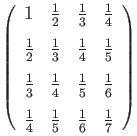
\includegraphics[width=0.2\textwidth]{./Images/H_4}
	\caption{Matrice de Hilbert de dimension 4}
\end{figure}

Le nombre d'étape pour trouver la solution sera en théorie inférieur ou égal à 4 (assuré par la méthode du gradient conjugué).\\

En notant $K_2(A)$ le conditionnement 2 de A tel que :\footnote{conditionnement obtenu sur Matlab}
$$K_2(a)= 1.5514*10^4$$

On a l'inégalité du conditionnement pour majorer l'erreur :
$$\frac{||\Delta x||_{2}}{||x||_2}\leq K_2(A)\frac{||\Delta b||_{2}}{||b||_2}$$

Le test d'arrêt est de la forme $$tol^2*(b,b) > (r,r) $$
avec $(\bullet,\bullet)$ le produit scalaire usuel et $tol=10^{-10}$.\\

Enfin, le vecteur $b$ est choisi comme ci-dessous :

$$b_i=\sum_{k=1}^4A_{ik}$$

de manière à avoir 
$$x^T=\left(\begin{array}{cccc}
1 & 1 & 1 & 1\end{array}\right)$$




\chapter{Vecteur résidu $r$} %thib

\section{Préambule}

Premier élément d'intérêt de notre projet, le vecteur résidu. Intéressons-nous aux erreurs faites par la machine sur ce vecteur. Nous ne reviendrons pas sur le rôle du vecteur résidu dans la méthode du gradient conjugué mais il est essentiel au bon fonctionnement de celle-ci.\\
Désormais, nous allons expliquer la démarche utilisée pour étudier cette erreur.

\begin{figure}[H]
	\center
	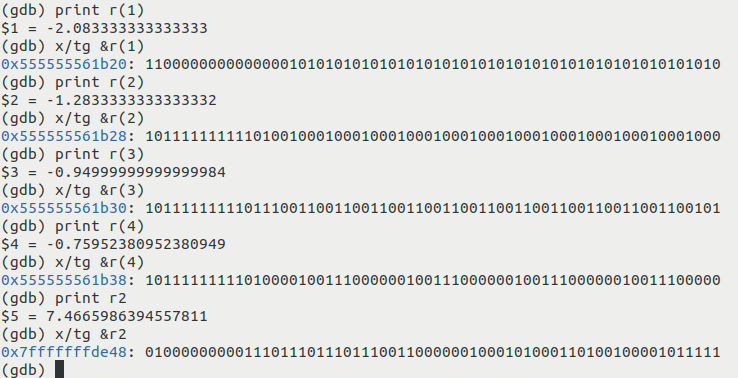
\includegraphics[width=1\textwidth]{./Images/Exemple_gdb}
	\caption{Capture d'écran avec le logiciel \textit{gdb}}
\end{figure}

Comme on peut le voir ci-dessus, nous avons utilisé le logiciel \textit{gdb} avec notre programme de gradient conjugué. On utilise le logiciel \textit{gdb} pour obtenir certaines valeurs pendant le déroulement du programme et pas uniquement à la fin. En ce qui nous concerne, nous récupérons les valeurs des composantes du vecteur résidu ainsi que leurs valeurs binaires qui seront importantes pour la suite. La composante r2 est la norme 2 au carré du vecteur résidu et c'est précisément ce que nous allons comparer avec notre calcul pour trouver l'erreur.\\

\begin{figure}[H]
	\center
	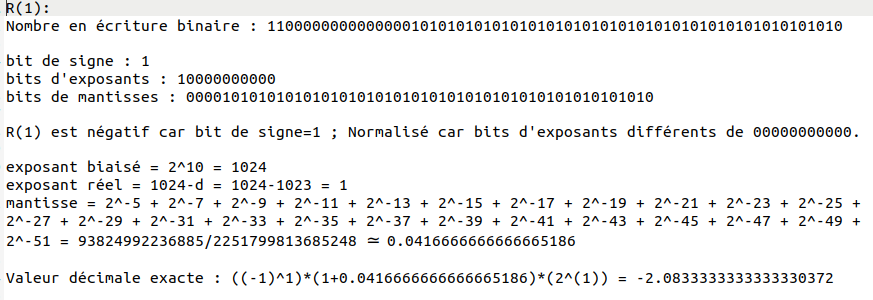
\includegraphics[width=1\textwidth]{./Images/r_0_dec}
	\caption{Conversion binaire réelle}
\end{figure}

Deuxième étape, on retrouve la valeur réelle en base 10 de notre nombre à partir de son écriture binaire en flottant.\\
On décompose le nombre par bits de signes, exposants et mantisses. On recalcule chacun des termes puis la valeur réelle finale grâce au logiciel en ligne \textit{wolframalpha}. \\
Maintenant que nous avons la valeur réelle de chaque composante nous allons pouvoir en déduire une valeur calculée par nous-même de r2 et la comparer avec celle donnée par l'ordinateur.\\
Nous allons maintenant voir cela à chaque itération du gradient conjugué et observer l'erreur absolue et relative entre la solution de l'ordinateur et la nôtre.


\section{Etape 0}

\begin{figure}[H]
	\center
	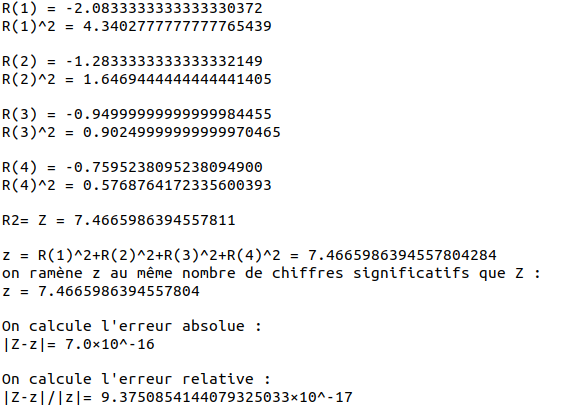
\includegraphics[width=0.9\textwidth]{./Images/r_0_err}
	\caption{Fichier d'erreur à l'étape 0}
\end{figure}

On peut voir que l'erreur absolue est de $10^{-16}$ et l'erreur relative de $10^{-17}$. On est autour de la précision machine pour une double précision et l'erreur relative reste extrêmement faible. On peut être plutôt satisfait du résultat.

\section{Etape 1}

\begin{figure}[H]
	\center
	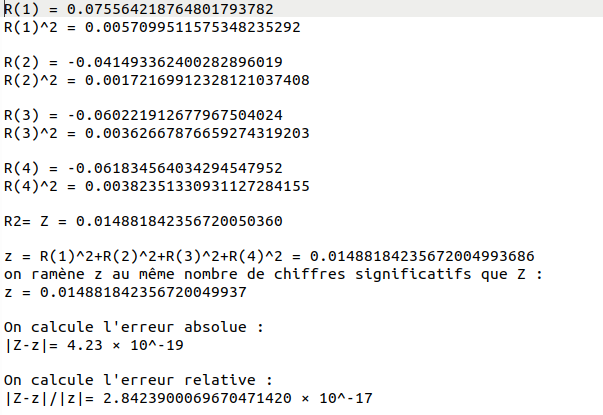
\includegraphics[width=0.9\textwidth]{./Images/r_1_err}
	\caption{Fichier d'erreur à l'étape 1}
\end{figure}

Cette fois l'erreur absolue est de $10^{-19}$ et la relative de $10^{-17}$ c'est même moins que l'étape d'avant.

\section{Etape 2}

\begin{figure}[H]
	\center
	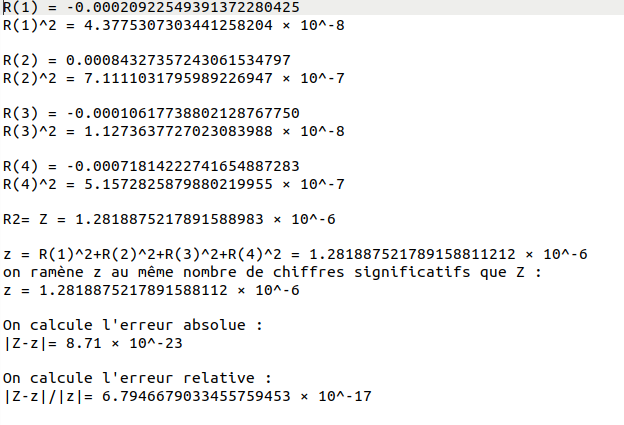
\includegraphics[width=0.9\textwidth]{./Images/r_2_err}
	\caption{Fichier d'erreur à l'étape 2}
\end{figure}

Une fois de plus, l'erreur absolue diminue elle est de $10^{-23}$. Cependant, quand on regarde l'erreur relative en $10^{-17}$, on se rend compte qu'elle n'a pas diminué.

\section{Etape 3}

\begin{figure}[H]
	\center
	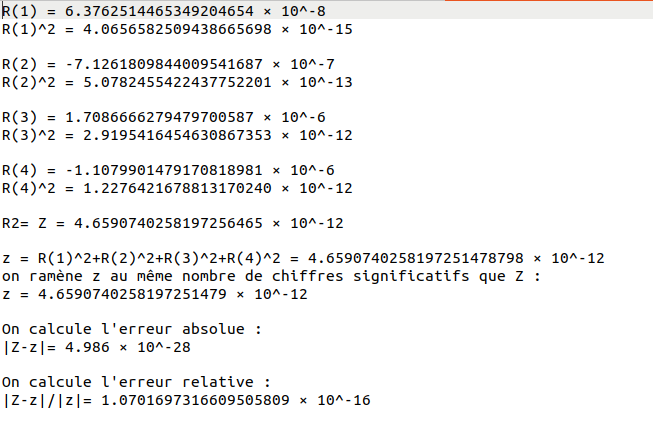
\includegraphics[width=0.9\textwidth]{./Images/r_3_err}
	\caption{Fichier d'erreur à l'étape 3}
\end{figure}

Encore on a une baisse de l'erreur absolue $10^{-28}$ mais l'erreur relative a tendance à remonter légèrement mais elle reste très faible.

\section{Etape 4}

\begin{figure}[H]
	\center
	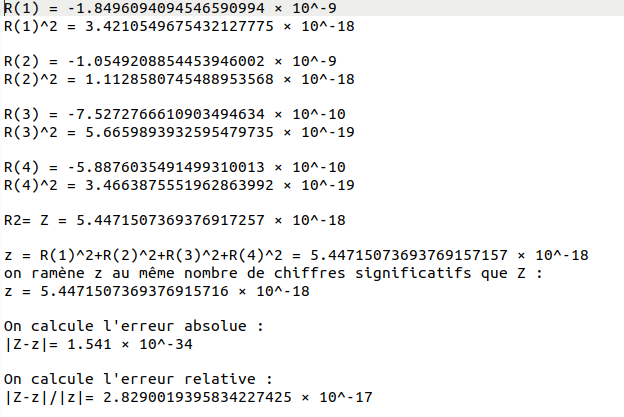
\includegraphics[width=0.9\textwidth]{./Images/r_4_err}
	\caption{Fichier d'erreur à l'étape 4}
\end{figure}

Nous avons une nouvelle fois une baisse de l'erreur absolue à $10^{-32}$. L'erreur relative reste quant à elle aux alentours de $10^{-17}$ comme depuis le début.

\section{postambule}

On a pu voir que l'erreur absolue avait tendance à diminuer et l'erreur relative à stagner autour de $10^{-17}$. Il est en fait logique que l'erreur absolue diminue car le vecteur résidu diminue à chaque itération du programme. C'est pourquoi il est souvent plus judicieux de regarder l'erreur relative qui est plus représentative.\\
A ce propos, elle est plutôt très faible et on peut être satisfait du résultat obtenu.

\chapter{Vecteur solution $x$} %kev

Intéressons-nous maintenant au vecteur solution $x$. On rappelle que la solution théorique attendue est le vecteur :
$$x^T=\left(\begin{array}{cccc}
1 & 1 & 1 & 1\end{array}\right)$$

Dans cette partie nous allons étudier les erreurs locales sur le vecteur solution $\hat{x}$ obtenu avec la méthode du gradient conjugué :
$$\hat{x}_{n+1}=\hat{x}_{n}-\alpha*p_n$$

avec
$$\alpha=\frac{(r_n,r_n)}{(Ap_n,p_n)}$$

On se propose d'étudier chaque composante du vecteur sur 4 étapes.

\section{Etape 1}

Pour chaque étape, on récupère les données en binaire grâce à \textit{gdb} puis on les stocke dans des fichiers comme ci-dessous :

\begin{figure}[H]
	\center
	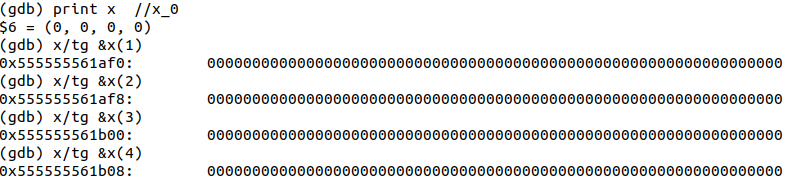
\includegraphics[width=0.9\textwidth]{./Images/gdb_x_0}
	\caption{Composantes de x à l'étape 0}
\end{figure}

\begin{figure}[H]
	\center
	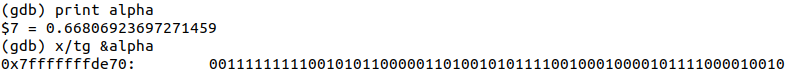
\includegraphics[width=0.9\textwidth]{./Images/gdb_alpha_0}
	\caption{Valeur de $\alpha$ à l'étape 0}
\end{figure}

\begin{figure}[H]
	\center
	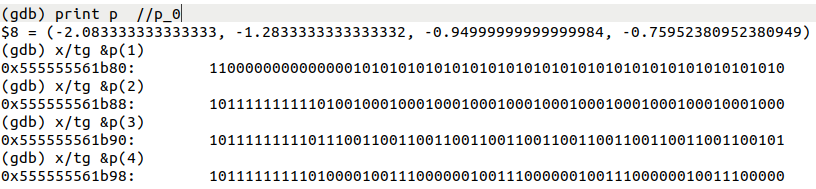
\includegraphics[width=0.9\textwidth]{./Images/gdb_p_0}
	\caption{Composantes de p à l'étape 0}
\end{figure}

\begin{figure}[H]
	\center
	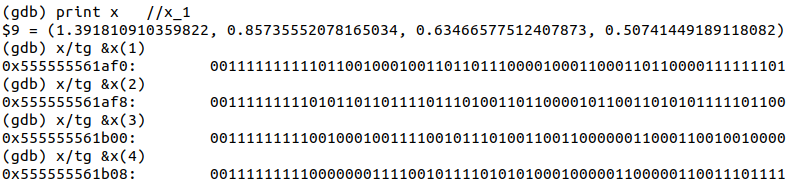
\includegraphics[width=0.9\textwidth]{./Images/gdb_x_1}
	\caption{Composantes de x à l'étape 1}
\end{figure}

Une fois les valeurs binaires obtenues, on peut alors calculer leur valeur. Soit par l'ordinateur, qui est en double précision donc qui aura des erreurs de l'ordre de $10^{-16}$, soit par un plus grand calculateur\footnote{\textit{wolframalpha.com}}, c'est ce qu'on se propose de faire.\\

On stocke également ces résultats dans des fichiers de manière à les comparer plus tard comme dans l'exemple ci-dessous :

\begin{figure}[H]
	\center
	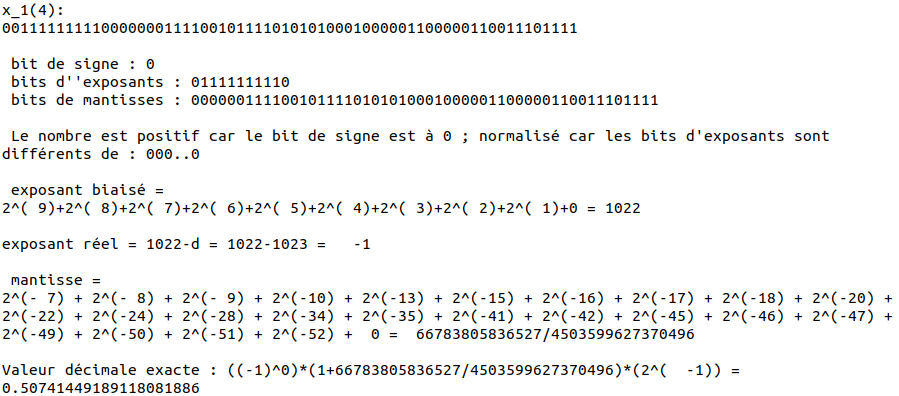
\includegraphics[width=0.9\textwidth]{./Images/x_1(4)}
	\caption{Calcul précis de la $4^{eme}$ composante de x à l'étape 1}
\end{figure}

Une fois le calcul précis de toutes les composantes de nos variables, on pourra alors comparer nos valeurs en local de manière à obtenir nos erreurs absolues et relatives. On obtient un fichier du type :

\begin{figure}[H]
	\center
	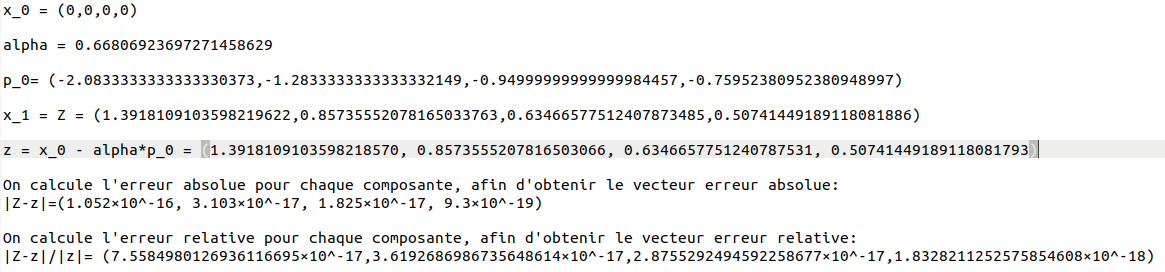
\includegraphics[width=0.9\textwidth]{./Images/err_x_1}
	\caption{Fichier erreur final obtenu pour l'étape 1}
\end{figure}

On s'intéresse seulement à ces deux lignes pour conclure :
\begin{figure}[H]
	\center
	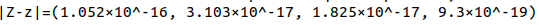
\includegraphics[width=0.5\textwidth]{./Images/err_abs_x_1}
	\caption{Vecteur erreur absolue pour l'étape 1}
\end{figure}
\begin{figure}[H]
	\center
	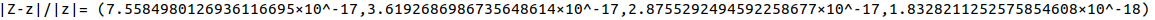
\includegraphics[width=1\textwidth]{./Images/err_rel_x_1}
	\caption{Vecteur erreur relative pour l'étape 1}
\end{figure}

On remarque que l'erreur relative pour toutes les composantes de $\hat{x}$ est inférieure à l'erreur machine $10^{-16}$ ce qui est plutôt bien, les calculs se sont bien passés informatiquement.

\section{Etape 2}

De même pour l'étape 2, on obtient les valeurs des différentes variables en binaire, nous calculons leur valeur exacte grâce à un calculateur\footnote{sur \textit{wolframalpha.com}} très performant afin d'avoir une très grande précision puis on compare le résultat final $Z$ que donne le programme avec celui calculé sur le calculateur $z$. On obtient ces résultats :

\begin{figure}[H]
	\center
	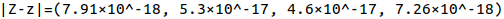
\includegraphics[width=0.5\textwidth]{./Images/err_abs_x_2}
	\caption{Vecteur erreur absolue pour l'étape 2}
\end{figure}
\begin{figure}[H]
	\center
	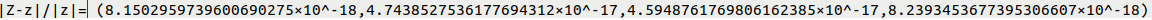
\includegraphics[width=1\textwidth]{./Images/err_rel_x_2}
	\caption{Vecteur erreur relative pour l'étape 2}
\end{figure}

Les erreurs sont de l'ordre de $10^{-18}$ bien inférieur à la précision machine $10^{-16}$. Les calculs se sont également bien passés.

\section{Etape 3}

Même chose pour l'étape 3, on obtient :

\begin{figure}[H]
	\center
	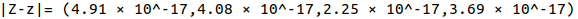
\includegraphics[width=0.5\textwidth]{./Images/err_abs_x_3}
	\caption{Vecteur erreur absolue pour l'étape 3}
\end{figure}
\begin{figure}[H]
	\center
	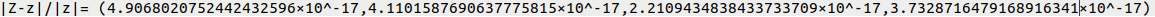
\includegraphics[width=1\textwidth]{./Images/err_rel_x_3}
	\caption{Vecteur erreur relative pour l'étape 3}
\end{figure}

Les erreurs sont cette fois-ci de l'ordre de $10^{-17}$, toujours inférieur à $10^{-16}$ ce qui indique que les calculs se sont bien passés.

\section{Etape 4}

Même démarche pour cette dernière étape, on obtient :

\begin{figure}[H]
	\center
	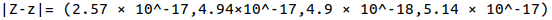
\includegraphics[width=0.5\textwidth]{./Images/err_abs_x_4}
	\caption{Vecteur erreur absolue pour l'étape 4}
\end{figure}
\begin{figure}[H]
	\center
	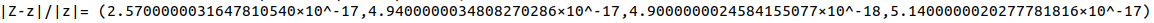
\includegraphics[width=1\textwidth]{./Images/err_rel_x_4}
	\caption{Vecteur erreur relative pour l'étape 4}
\end{figure}

Les erreurs sont de l'ordre de $10^{-17}$ une nouvelle fois, on conclut alors que l'ensemble des calculs pour les 4 étapes se sont bien déroulés informatiquement.

\chapter{Analyse numérique du problème} %kev

Analysons maintenant le problème numériquement. On sait que la solution théorique est
$$x^T=\left(\begin{array}{cccc}
1 & 1 & 1 & 1\end{array}\right)$$

Comparons maintenant ce résultat avec celui qu'on a obtenu numériquement au bout de la $4^{eme}$ étape :
$$\hat{x}^T=\left(\begin{array}{cccc}
0.9999999987685677105 & 0.9999999992953791939 & 0.9999999994982825546 & 0.99999999960549057491\end{array}\right)$$\vspace{0cm}

On peut maintenant obtenir l'erreur absolue pour chaque composante afin d'obtenir le vecteur absolu :\footnote{calcul effectué sur \textit{wolframalpha.com}}

$$\varepsilon_{abs}=\left(\begin{array}{cccc}
1.2314322895*10^{-9} & 7.046208061*10^{-10} & 5.017174454*10^{-10} & 3.9450942509*10^{-10} \end{array}\right)$$\vspace{0cm}

On remarque que l'on obtient le même vecteur pour le vecteur erreur relative puisqu'on divise toutes les composantes par 1 :

$$\varepsilon_{rel}=\left(\begin{array}{cccc}
1.2314322895*10^{-9} & 7.046208061*10^{-10} & 5.017174454*10^{-10} & 3.9450942509*10^{-10} \end{array}\right)$$

On observe des erreurs beaucoup plus élevées que celles obtenues localement. En effet, pour une étude locale, on obtenait des erreurs d'ordre de grandeur d'environ $10^{-17}$ alors qu'ici il est d'environ $10^{-10}$. Une différence de $10^{7}$ qui n'est pas négligeable.\\

Cependant, on peut souligner l'efficacité de la méthode car en seulement 4 itérations, l'erreur de la solution obtenue par rapport à celle théorique est de seulement $10^{-9}$. Si l'on veut obtenir plus de précision, il suffit de diminuer la tolérance et d'observer davantage d'étapes.





\chapter*{Conclusion} %thib
\addcontentsline{toc}{chapter}{Conclusion}

Pour conclure, on a pu observer l'évolution de l'erreur absolue et de l'erreur relative sur deux éléments différents : le vecteur résidu et le vecteur x. On a constaté en général des résultats plutôt satisfaisants sur les deux éléments concernant la différence entre le résultat obtenu par machine et celui obtenu par un calcul manuel sensé servir de référence.\\

Premièrement, concernant le vecteur résidu. Tout d'abord on rappelle que le vecteur résidu a normalement tendance à diminuer en norme et il est même bien souvent important dans la condition d'arrêt. Nous avons remarqué une erreur absolue qui diminue, ce qui est logique car le vecteur converge. Cependant au niveau de l'erreur relative on a observé une stagnation autour de $10^{-17}$ ce qui est très satisfaisant, la précision machine étant de $10^{-16}$ en double précision. On peut donc conclure que le calcul s'est plutôt bien passé informatiquement.\\

Deuxièmement, par rapport au vecteur x. Ce dernier tend vers la solution théorique du système linéaire : le vecteur unitaire. On remarquera que la solution x final n'est pas exactement égale à la solution théorique mais c'est un autre sujet où le critère de tolérance a son importance. Dans notre cas, nous avons seulement comparé le résultat de la machine et celui calculé de notre côté. On peut voir que l'erreur reste toujours inférieure à $10^{-16}$ ce qui est la précision machine en double précision. On en conclut que les résultats sont très satisfaisants. \\

Pour finir, on peut résumer en disant que l'ensemble des calculs se sont bien déroulés informatiquement sur l'ensemble des flottants. Néanmoins, rien ne nous garantit qu'avec une autre méthode ou une autre matrice on aurait obtenu la même chose. Il serait intéressant de mener la même étude avec d'autres matrices plus grandes au conditionnement élevé et en variant les méthodes.


\end{document}
